\documentclass[TheoreticalPhy_ModB.tex]{subfiles}
\begin{document}


\chapter{QED Processes at Lowest order} %Sei stato bravissimo, si chiamava proprio così

\section{The QED Lagrangian and its Symmetries}
\textsf{Mandl, sec 11.1 - Maggiore, sec 7.1}\\
Quantum electrodynamic (QED) describes the interactions between (or any other charged spin 1/2 particle) and photons. QED is described by the lagrangian
\[
\mathL_{\text{QED}} =\underbrace{\overline{\psi }( i\slashed \partial -m) \psi }_{\mathcal{L}^{( 0)}_{D}} \ -\underbrace{\frac{1}{4} F_{\mu \nu } F^{\mu \nu }}_{\mathcal{L}_{EM}} -\underbrace{qA_{n}\overline{\psi } \gamma ^{\mu } \psi }_{\mathcal{L}_{int}} -\underbrace{\frac{1}{2\xi }\left( \partial _{\mu } A^{\mu }\right)^{2}}_{\mathcal{L}_{GF}}
%Vengono un po' una merda le graffe sotto quindi vedi tu se vuoi tenerele o fare in un altro modo
\]
\begin{enumerate}
\item $\mathL_D^{(0)}$ is the langrangian for the free Dirac field
\item $\mathL_{EM}$ is the lagrangian for the free EM field. In order to quatize the E-n field we have to add the term $\mathL_{GF}$ (gauge fixing). For other purposes this term can be omitted. Usually the choice $\xi = 1$, called Feynman gauge, is the simplest choice for quantization
\item $\mathL_{int}$ describes the interaction between Dirac field and EM-field. Notice that the term $\mathL_D = \mathL_D^{(0)} + \mathL_{int}$ can be obtained from $\mathL_D^{(0)}$ with the ``minimal substitution'' $\partial_{\mu} \to \partial_{\mu} + iqA_{\mu} = D_{\mu}$, i.e. using covariant derivative $D_{\mu}$ instead of $\partial_{\mu}$ in the dirac lagrangian.\\
Notice that $\mathL_D$ exhibits local symmetry, while $\mathL_D^{(0)}$ doesn't
\end{enumerate}
Besides Lorentz invariance, the QED exhibits following symmetries:
\begin{enumerate}[label=(\Roman*)]
\item \textbf{Global U(1) symmetry}
\[
\begin{cases}
\psi(x) \to \psi'(x) = e^{i \alpha}\psi(x) \qquad \alpha \in \mathR \\
A^{\mu}(x) \to A^{\prime \mu}(x) = A^{\mu}(x)
\end{cases}
\]
There is therefore an associated conserved Noether current
\[
j^{\mu} = q \overline{\psi} \gamma^{\mu} \psi
\quad \to \quad
\partial_{\mu}j^{\mu} = 0 
\]
and a U(1) charge which is conserved by the EM interaction
\[
Q = q \int \de^3 x \ \psi^{\dagger} \psi
\qquad
\frac{\de Q}{\de t} = 0
\]
\item \textbf{Local U(1) symmetry} (gauge symmetry)
\[
\begin{cases}
\psi(x) \to \psi'(x) = e^{iq\alpha(x)} \psi(x) \\
A^{\mu} \to A^{\prime \mu}(x) = A^{\mu}(x) - iq\partial^{\mu}\alpha(x)
\end{cases}
\]
notice that the global U(1) symmetry is a sequence of the local U(1) symmetry, taking $\alpha(x)$ constant)\\ \\
The covariant derivative of $\psi$ $D_{\mu}\psi$ behaves as a spinor (remember that $D_{\mu}$ transforms as a vector):
\[
\begin{split}
D_{\mu}\psi \to (D_{\mu}\psi)' = D'_{\mu}\psi'	& = (D_{\mu} - iq\partial_{\mu} \alpha)(e^{iq\alpha(x)} \psi(x)) \\
	& = (\partial_{\mu} + iqA_{\mu} - iq\partial_{\mu}\alpha)(e^{iq\alpha} \psi) \\
	& = e^{iq\alpha}(\partial_{\mu} + iqA_{\mu})\psi \\
	& = e^{iq\alpha(x)}(D_{\mu}\psi)
\end{split}
\]
This implies that $\mathL_D$ is invariant. Since $\mathL_{EM}$ is invariant, the full lagrangian is invariant
\end{enumerate}

\section{Flavors in QED and the SU(3) Flavor Global Symmetry}
QED describes interactions of the photon field with several kind of leptons, not only electron and positrons. Particles that differs only by their mass are called \textbf{flavours}.
\skipline
The next table describes leptons in QED. There are two families of leptons that differs by their charge. We indicate with (-) (minus) particles with negative charge, and with (+) (plus) particles with positive charge (antiparticles)\\
\skipline
Flavours in QED
\[
\begin{array}{l | cccccc}
\toprule
Leptons \footnotemark	& e 		& \mu 	& \tau 	& \nu_e 		& \nu_{\mu} 	& \nu_{\tau} \\
\midrule
q					& -1		& -1		& -1		& 0			& 0			& 0 \\
m [MeV]				& 0.5		& 105	& 1777	& \simeq 0		& \simeq 0		& \simeq 0 \\
\bottomrule
\end{array}
\]
\footnotetext{Neutrinos admit anly global U(l) symmetry \\
Neutrino masses are in the order $m_{\nu} \approx 10^{-6} me \le 1 eV$}
\skipline
The dirac lagrangian $\mathL_D$ can be modified in order to consider all possible leptons
\[
\mathL_D = \sum_{i=1}^n \bar{\psi_i} (i \slashed D - m_i) \psi_i
	\simeq \sum_{i=1}^{n_l} \bar{\psi_i} (i \slashed D - m_i) \psi_i
	+ \sum_{j=1}^{n_n} \bar{\psi_i} (i \slashed \partial) \psi_i
\]
with $n$: number of leptons, $n_l$: number of electrically charged particles, $n_n$: number of neutrinos.\\
In the last term the interaction term vanishes because of q=0\\
If we adopt a matrix notation
\begin{align}
\Psi_C & =
\begin{pmatrix}
\psi_e \\
\psi_{\mu} \\
\psi_{\tau}
\end{pmatrix}
&
\Psi_N & =
\begin{pmatrix}
\psi_{\nu_e} \\
\psi_{\nu_{\mu}} \\
\psi_{\nu_{\tau}}
\end{pmatrix}
\notag \\
\bar{\Psi}_C & = (\bar{\psi_e}, \bar{\psi_{\mu}}, \bar{\psi_{\tau}})
&
\bar{\Psi}_N & = (\bar{\psi}_{\nu_e}, \bar{\psi}_{\nu_{\mu}}, \bar{\psi}_{\nu_{\tau}})
\notag 
\end{align}
The subscript C stands for ``charged'', and N for ``neutral''\\
We can define following matrices
\[
M_C =
\begin{pmatrix}
m_e 	& 0 			& 0 \\
0	& m_{\mu}	& 0 \\
0	& 0			& m_{\tau}
\end{pmatrix}
\qquad
Q_C = (-1) \mathds{1}_{3 \times 3}
\qquad
M_N \simeq Q_N = \emptyset_{3 \times 3}
\]
and the generalization of the covariant derivative $D_{\mu} = \partial_{\mu} \cdot \mathds{1}_{3 \times 3} + iA_{\mu}Q_C$ we obtain
\[
\mathL_D = \underbrace{\bar{\Psi}_C (i \slashed D - M_C)\Psi_C}_{\mathL_C} +
	\underbrace{\bar{\Psi}_N(i \slashed \partial \mathds{1}_{3 \times 3})\Psi_N}_{\mathL_N}
\]

\section{$e^-\gamma\rightarrow e^-\gamma$ (Compton)}
\textsf{See Peskin, sec 5.5}\\
Let's examinate a process with external bosons: \emph{Compton scattering}, or $e^-\gamma\rightarrow e^-\gamma$. This process is described by two independent diagrams, since they are topologically different:

\begin{equation*}\mathcal M_A=%
\begin{tikzpicture}[baseline=(nu)]
  \begin{feynman}[large]
    \vertex (f1) {\(e^-_{(r)}\)};
    \vertex [label={[label distance=0.1cm]180:$\nu$}] at ([shift={(315:2.5)}]f1) (nu);
    \vertex [below left=of nu] (b1) {\(\gamma_{(\lambda)}\)};
    \vertex [label={[label distance=0.12cm]2:$\mu$}] at ([shift={(0:3.2)}]nu) (mu);
    \vertex [above right=of mu] (f2) {\(e^-_{(r')}\)};
    \vertex [below right=of mu] (b2) {\(\gamma_{(\lambda')}\)};

    \diagram*{
      (f1) -- [fermion, momentum={[arrow shorten=0.2]\(p\)}] (nu) -- [fermion, momentum={[arrow shorten=0.3]\(q=p+k=\sqrt{s}\)}] (mu) -- [fermion, momentum={[arrow shorten=0.2]\(p'\)}] (f2),
      (b1) -- [boson, momentum'={[arrow shorten=0.25]\(k\)}] (nu),
      (mu) -- [boson, momentum'={[arrow shorten=0.25]\(k'\)}] (b2),
    };
  \end{feynman}
\end{tikzpicture}
\end{equation*}

\begin{equation*}\mathcal M_B=\,
\begin{tikzpicture}[baseline=(mu)]
  \begin{feynman}[large]
    \vertex (f1) {\(e^-_{(r)}\)};
    \vertex [label={[label distance=0.1cm]180:$\mu$}] at ([shift={(315:2.5)}]f1) (mu);
    \vertex [label={[label distance=0.1cm]0:$\nu$}] at ([shift={(0:3.4)}]mu) (nu);
    \vertex [above right=of nu] (f2) {\(e^-_{(r')}\)};
    \vertex at ([shift={(270:3.2)}]f1) (b1){\(\gamma_{(\lambda)}\)};
    \vertex at ([shift={(270:3.4)}]f2) (b2){\(\gamma_{(\lambda')}\)};
    
    \diagram*{
      (f1) -- [fermion, momentum={[arrow shorten=0.2]\(p\)}] (mu) -- [fermion, momentum={[arrow shorten=0.3]\(q=p-k'=\sqrt{u}\)}] (nu) -- [fermion, momentum={[arrow shorten=0.2]\(p'\)}](f2),
      (mu) -- [boson, momentum'={[shift={(345:0.7)}, arrow shorten=0.4]\(k'\)}] (b2),
      (b1) -- [boson, momentum'={[shift={(200:0.6)}, arrow shorten=0.4]\(k\)}] (nu),
      };
  \end{feynman}
\end{tikzpicture}
\quad=
\begin{tikzpicture}[baseline=(i)]
  \begin{feynman}[large]
    \vertex (f1) {\(e^-_{(r)}\)};
    \vertex [label={[label distance=0cm]182:$\mu$}] at ([shift={(315:2.5)}]f1)  (mu);
    \vertex [label={[label distance=0.1cm]270:$\nu$}] at ([shift={(270:2)}]mu) (nu);
    \vertex [below right=of nu] (f2) {\(e^-_{(r')}\)};
    \vertex [below left=of nu] (b1){\(\gamma_{(\lambda)}\)};
    \vertex [above right=of mu] (b2){\(\gamma_{(\lambda')}\)};
    \vertex at ([shift={(270:1)}]mu)(i);
    
    \diagram*{
      (f1) -- [fermion, momentum={[arrow shorten=0.25]\(p\)}] (mu) -- [fermion, momentum={[arrow shorten=0.3]\(q=p-k'=\sqrt{u}\)}] (nu) -- [fermion, momentum={[arrow shorten=0.2]\(p'\)}](f2),
      (mu) -- [boson, momentum={[arrow shorten=0.3]\(k'\)}] (b2),
      (b1) -- [boson, momentum={[arrow shorten=0.2]\(k\)}] (nu),
      };
  \end{feynman}
\end{tikzpicture}
\end{equation*}

{\small We wrote the diagram of $\mathcal M_B$ in two topologically equivalent forms: in the first one is clear the topological relation with diagram of $\mathcal M_A$ (this is useful to find the relative sign between diagrams $A$ and $B$: it's clear that diagrams differs for the permutation of two bosons), while in the second one is clear that it describes a $u$-channel.}

\skipline
Amplitudes reads, using Feynman rules

\begin{align*}
\mathcal M_A&=\bar u_{r'}(p')(-iq\gamma^\mu)\epsilon_\mu^{\lambda'*}(k')\tilde S_F(p+k)(-iq\gamma^\nu)\epsilon_\nu^\lambda(k)u_r(p)\\
&=-q^2\epsilon_\mu^{\lambda'*}(k')\epsilon_\nu^\lambda(k)\left[\bar u_{r'}(p')\gamma^\mu\tilde S_F(p+k)\gamma^\nu u_r(p)\right]\\
&\,\\
\mathcal M_B&=-q^2\epsilon_\mu^{\lambda'*}(k')\epsilon_\nu^\lambda(k)\left[\bar u_{r'}(p')\gamma^\nu\tilde S_F(p-k')\gamma^\mu u_r(p)\right]
\end{align*}

{\small (Recall that $\tilde S_F$ is a matrix, so elements in the squared braket  must be written in this order)}\\
Because of anticommuting relations for bosons, these amplitudes must be summed up in the total amplitude.
The explicit form of Feynman propagator for the Dirac field reads

\[\tilde S_F(p)=\frac{i(\slashed p+m)}{p^2-m^2+i\epsilon}=\frac i{\slashed p-m+i\epsilon}\]
so total amplitude is

\[\mathcal M=-iq^2\epsilon_\mu^{\lambda'*}(k')\epsilon_\nu^\lambda(k)\bar u_{r'}(p')\left[\frac{\gamma^\mu(\slashed p+\slashed k+m)\gamma^\nu}{(p+k)^2-m^2}+\frac{\gamma^\nu(\slashed p-\slashed k'+m)\gamma^\mu}{(p-k')^2-m^2}\right]u_r(p)\]

We make some simplifications before squaring  this expression. Since $p^2=m^2$ and $k^2=0$:
\[(p+k)^2-m^2=2p\cdot k\qquad(p-k')^2-m^2=-2p\cdot k'\]

To simplify numerators, I can use Dirac algebra:
\begin{align*} 
(\slashed p+m)\gamma^\nu u(p)&=(p_\mu\gamma^\mu\gamma^\nu+m\gamma^\nu)u(p)=(2g^{\mu\nu}p_\mu-p_\mu\gamma^\nu\gamma^\mu+m\gamma^\nu)u(p)\\
&=2p^\nu u(p)-\gamma^\nu\underbrace{(\slashed p-m)}_{2m\,\Lambda_-(p)}u(p)=2p^\nu u(p)
\end{align*}

Using these tricks we obtain

\[\mathcal M = -iq^2\epsilon_\mu^{\lambda'*}(k')\epsilon_\nu^\lambda(k)\bar u_{r'}(p')\left[\frac{\gamma^\mu\slashed k\gamma^\nu+2\gamma^\mu p^\nu}{2p\cdot k}+\frac{-\gamma^\nu\slashed k'\gamma^\mu+2\gamma^\nu p^\mu}{-2p\cdot k'}\right]u_r(p)\]

\subsection{The Ward Identities and sum over the photon polarizations}
\textsf{See Mandl, sec 8.3}\\
The next step in the calculation will be to square this expression for $\mathcal M$ and sum or average over electron and photon polarization states. The sum over electron polarizations can be performed as before, using $\sum u(p)\bar u(p)=\slashed p+m$. Fortunately, there is a similar trick for summing over photons polarization vectors.\\
Gauge invariance of the theory implies the gauge invariance of the matrix elements, i.e. of the Feynman amplitudes. It is, of course, only the matrix element itself, corresponding to the sum of all possible Feynman graphs in a given order of perturbation theory, which must be gauge invariant. For example, for the Compton scattering, the individual amplitudes $\mathcal A$ and $\mathcal B$ are not gauge invariants, but their sum $\mathcal M$ is.\\
For any process involving external photons, the Feynman amplitude $\mathcal M$ is of the form
\begin{equation}\label{eqn:Ward-form}
\mathcal M=\epsilon_\alpha^{\lambda_1}(k_1)\epsilon_\beta^{\lambda_2}(k_2)\dots L^{\alpha\beta\dots}(k_1,k_2,\dots)
\end{equation}
with one polarization vector $\epsilon^{\lambda_i}(k_i)$ for each external photon, and the tensor amplitude $L^{\alpha\beta\dots}(k_1,k_2,\dots)$ independent of these polarization vectors.\\
The polarization vectors are of course gauge dependent. For example, for a free photon described in the Lorentz gauge by the plane wave
\[A^\mu(x)=\textup{const}\,\cdot\epsilon_\lambda^\mu(k)e^{\pm ikx}\]
the gauge transformation
\[A^\mu\rightarrow A'^\mu(x)=A^\mu(x)+\partial^\mu\alpha(x)\qquad\textup{with}\quad \alpha(x)=\tilde\alpha(k)e^{\pm ikx}\]
implies
\[\epsilon_\lambda^\mu(k)\rightarrow{\epsilon'}_\lambda^{\mu}(k)=\epsilon_\lambda^\mu(k)\pm ik^\mu\tilde\alpha(k)\]
Invariance of the amplitude Eq.\eqref{eqn:Ward-form} under this transformation requires
\[k^\alpha_1L_{\alpha,\beta,\dots}(k_1,k_2,\dots)=k^\beta_1L_{\alpha,\beta,\dots}(k_1,k_2,\dots)=\dots=0\]
i.e. when any external photon polarization vector is replaced by the corresponding four momentum, the amplitude must vanish. This is the statement of the \emph{Ward Identity}:

\todo{Sistemare grafica}%%%%%%%%%%%

\begin{quoting}
If $\mathcal M(k)=\epsilon_\mu(k)L^\mu(k)$ is the amplitude for some QED process involving an external photon with momentum $k$, then this amplitude vanishes if we replace $\epsilon_\mu$ with $k_\mu$:
\[k_\mu L^\mu(k)=0\]
\end{quoting}

\todo{Creare ambiente exercize, questo è un esercizio}
\begin{example}
Verify explicitly the Ward Identity for the Feynman amplitude of Compton scattering
\end{example}

\textsf{See Peskin, sec 5.5}\\
Returning to our derivation of the polarization sum formula for squared scattering amplitude. Writing in general
\[\mathcal M=\epsilon_\mu^{(\lambda)}(k)L^\mu(k)\]
then the sum over polarizations of the photon with momentum $k$ reads
\[\sum_{\lambda=1,2}|\mathcal M|^2=\sum_{\lambda=1,2}\epsilon_\mu^{(\lambda)}(k)\epsilon_\nu^{(\lambda)*}(k)L^\mu(k)L^{\nu\dagger}(k)\]
Because of the covariance of the theory we can do the calculation in a specific frame. In order to simplify the analysis we choose the frame where the photon moves along the $\hat z$ axis:
\[k^\mu=(|k|,0,0,|k|)\]
In this case the Ward Identity reads
\[0=k_\mu L^\mu=|k|\left(L^0-L^3\right)\qquad\longrightarrow\qquad L^0=L^3\]
Recall that in this frame
\[\epsilon_\mu^{(1)}(k)=(0,1,0,0)\qquad\epsilon_\mu^{(2)}(k)=(0,0,1,0)\]

So we have
\begin{align*}\sum_{\lambda=1,2}\epsilon_\mu^{(\lambda)}(k)\epsilon_\nu^{(\lambda)*}(k)L^\mu(k)L^{\nu\dagger}(k)&=\abs{L^1}^2+\abs{L^2}^2=\abs{L^1}^2+\abs{L^2}^2+\abs{L^3}^2-\abs{L^0}^2=-g_{\mu\nu}L^\mu L^\nu
\end{align*}
So we obtained the general rule to simplify photons polarization sum\footnote{Notice that we could prove (see Peskin) that even if we took $\lambda=0,1,2,3$, we could have obtained that the unphysical time-like and longitudinal photons can be consistently omitted from QED calculations, since in any event the squared amplitudes for producing these states cancel to give zero total probability. }
\todo{Creare ambiente per riquadrare le formule}
\[\sum_{\lambda=1,2}\epsilon_\mu^{(\lambda)}(k)\epsilon_\nu^{(\lambda)*}(k)L^\mu(k)L^{\nu\dagger}(k)\quad\longrightarrow\quad-g_{\mu\nu}\]




\subsection{The Klein-Nishima formula and the Thomson scattering}
\textsf{See Peskin, sec. 5.5}\\

To obtain the unpolarized cross section for Compton scattering, we use the covariant method described in the previous section. Writing
\[\mathcal M=\epsilon_\mu^{\lambda'*}(k')\epsilon_\nu^\lambda(k)\left(L^{\mu\nu}(k,k')\right)_{r,r'}\]
with 
\[\left(L^{\mu\nu}(k,k')\right)_{r,r'}=-iq^2\bar u_{r'}(p')\left[\frac{\gamma^\mu\slashed k\gamma^\nu+2\gamma^\mu p^\nu}{2p\cdot k}+\frac{-\gamma^\nu\slashed k'\gamma^\mu+2\gamma^\nu p^\mu}{-2p\cdot k'}\right]u_r(p)\]
we obtain
\begin{align*}
|\bar{\mathcal M}|^2&=\frac14\left(\sum_{\lambda'}\epsilon_\mu^{(\lambda')*}(k')\epsilon_\rho^{(\lambda')}(k')\right)\left(\sum_{\lambda}\epsilon_\nu^{(\lambda)*}(k)\epsilon_\sigma^{(\lambda)}(k')\right)\sum_{r,r'}\left(L^{\mu\nu}\right)_{r,r'}\left(L^{\rho\sigma}\right)^\dagger_{r,r'}\\
&=\frac14g_{\mu\rho}g_{\nu\sigma}\sum_{r,r'}\left(L^{\mu\nu}\right)_{r,r'}\left(L^{\rho\sigma}\right)^\dagger_{r,r'}
=\frac14\left(L^{\mu\nu}\right)_{r,r'}\left(L_{\mu\nu}\right)^\dagger_{r,r'}\\
&=\frac{q^4}4\Tr\Bigg[(\slashed p'+m)\left(\frac{\gamma^\mu\slashed k\gamma^\nu+2\gamma^\mu p^\nu}{2p\cdot k}+\frac{\gamma^\nu\slashed k'\gamma^\mu-2\gamma^\nu p^\mu}{2p\cdot k'}\right)\times\\
&\qquad\qquad\times(\slashed p+m)\left(\frac{\gamma_\nu\slashed k\gamma_\mu+2\gamma_\mu p_\nu}{2p\cdot k}+\frac{\gamma_\mu\slashed k'\gamma_\nu-2\gamma_\nu p_\mu}{2p\cdot k'}\right)\Bigg]\\
&=\frac{q^4}4\left\{\frac{T_{AA}}{(2p\cdot k)^2}+\frac{T_{BB}}{(2p\cdot k')^2}+\frac{T_{AB}+T_{BA}}{(2p\cdot k)(2p\cdot k')}\right\}
\end{align*}
where
\begin{align*}
T_{AA}&=\Tr\left[(\slashed p'+m)(\gamma^\mu\slashed k\gamma^\nu+2\gamma^\mu p^\nu)(\slashed p+m)(\gamma_\nu\slashed k\gamma_\mu+2\gamma_\mu p_\nu)\right]\\
T_{BB}&=\Tr\left[(\slashed p'+m)(\gamma^\nu\slashed k'\gamma^\mu-2\gamma^\nu p^\mu)(\slashed p+m)(\gamma_\mu\slashed k'\gamma_\nu-2\gamma_\nu p_\mu)\right]\\
T_{AB}&=\Tr\left[(\slashed p'+m)(\gamma^\mu\slashed k\gamma^\nu+2\gamma^\mu p^\nu)(\slashed p+m)(\gamma_\mu\slashed k'\gamma_\nu-2\gamma_\nu p_\mu)\right]\\
T_{BA}&=\Tr\left[(\slashed p'+m)(\gamma^\nu\slashed k'\gamma^\mu-2\gamma^\nu p^\mu)(\slashed p+m)(\gamma_\nu\slashed k\gamma_\mu+2\gamma_\mu p_\nu)\right]
\end{align*}

Notice that $T_{BB}=T_{AA}(k\leftrightarrow -k')$ and $T_{BA}=T_{AB}(k\leftrightarrow -k')$, we need therefore only calculate $T_{AA}$ and $T_{AB}$.\\
Considering $T_{AA}$, there are 16 terms inside the trace, but half contains an odd number of $\gamma$ matrices and therefore vanishes. Other terms are
\begin{align*}
\circled 1&=\Tr[\slashed p'\gamma^\mu\slashed k\gamma^\nu\slashed p\gamma_\nu\slashed k\gamma_\mu]\\
\circled 2&=2\Tr[\slashed p'\gamma^\mu\slashed k\gamma^\nu\slashed p\gamma_\mu p_\nu]
=2\Tr[\slashed p'\gamma^\mu\slashed k\slashed p\slashed p\gamma_\mu]\\
\circled 3&=2\Tr[\slashed p'\gamma^\mu p^\nu\slashed p\gamma_\nu\slashed k\gamma_\mu]
=2\Tr[\slashed p'\gamma^\mu \slashed p\slashed p\slashed k\gamma_\mu]\\
\circled 4&=4\Tr[\slashed p'\gamma^\mu p^\nu\slashed p\gamma_\mu p_\nu]
=4p^2\Tr[\slashed p'\gamma^\mu \slashed p\gamma_\mu]\\
\circled 5&=m^2\Tr[\gamma^\mu\slashed k\gamma^\nu\gamma_\nu\slashed k\gamma_\mu]\\
\circled 6&=2m^2\Tr[\gamma^\mu\slashed k\gamma^\nu\gamma_\mu p_\nu]
=2m^2\Tr[\gamma^\mu\slashed k\slashed p\gamma_\mu]\\
\circled 7&=2m^2\Tr[\gamma^\mu p^\nu\gamma_\nu\slashed k\gamma_\mu]
=2m^2\Tr[\gamma^\mu \slashed p\slashed k\gamma_\mu]\\
\circled 8&=4m^2\Tr[\gamma^\mu p^\nu\gamma_\mu p_\nu]
=4m^2p^2\Tr[\gamma^\mu \gamma_\mu ]\\
\end{align*}

In order to simplify above formulas we recall the proprieties of contractions of $\gamma$ matrices, i.e. products in the form $\gamma^\mu A\gamma^\mu$ where $A$ is a matrix:

\begin{enumerate}
\item $\gamma^\mu\gamma_\mu=4\id$
\item $\gamma^\mu\slashed p\gamma_\mu=-2\slashed p$
\item $\gamma^\mu\slashed p\slashed q\gamma_\mu=4p\cdot q$
\item $\gamma^\mu\slashed p\slashed q\slashed k\gamma_\mu=-2\slashed k\slashed q\slashed p$
\end{enumerate}

Using these proprieties, cyclicity of the trace and anticommuting proprieties of gamma matrices\footnote{$\slashed A\slashed B=A_\mu B_\nu\gamma^\mu\gamma^\nu=A_\mu B_\nu(2g^{\mu\nu}\id-\gamma^\nu\gamma^\mu)=2(A\cdot B)\,\id-\slashed B\slashed A\qquad\rightarrow\qquad\slashed A\slashed A=A^2\,\id$

$\Tr[\slashed A\slashed B]=2(A\cdot B)\,\Tr[\id]-\Tr[\slashed B\slashed A]=8(A\cdot B)-\Tr[\slashed A\slashed B]\qquad\rightarrow\qquad\Tr[\slashed A\slashed B]=4(A\cdot B)\id$}, we obtain (remember that $p^2=m^2$ and $k^2=0$):

\begin{align*}
\circled 1&=\Tr[\slashed p'\gamma^\mu\slashed k\gamma^\nu\slashed p\gamma_\nu\slashed k\gamma_\mu]
=-2\Tr[\slashed p'\gamma^\mu\slashed k\slashed p\slashed k\gamma_\mu]
=4\Tr[\slashed p'\slashed k\slashed p\slashed k]
=-4\Tr[\slashed p'\slashed k^2\slashed p]+8(p\cdot k)\Tr[\slashed p'\slashed k]
=32(p\cdot k)(p'\cdot k)\\
\circled 2&=2\Tr[\slashed p'\gamma^\mu\slashed k\slashed p\slashed p\gamma_\mu]
=-4\Tr[\slashed p'\slashed p\slashed p\slashed k]
=-4m^2\Tr[\slashed p'\slashed k]
=-16m^2(p'\cdot k)\\
\circled 3&=2\Tr[\slashed p'\gamma^\mu \slashed p\slashed p\slashed k\gamma_\mu]
=2m^2\Tr[\slashed p'\gamma^\mu \slashed k\gamma_\mu]
=-4m^2\Tr[\slashed p'\slashed k]
=-16m^2(p'\cdot k)\\
\circled 4&=4p^2\Tr[\slashed p'\gamma^\mu \slashed p\gamma_\mu]
=-8m^2\Tr[\slashed p'\slashed p]=-32m^2(p'\cdot p)\\
\circled 5&=m^2\Tr[\gamma^\mu\slashed k\gamma^\nu\gamma_\nu\slashed k\gamma_\mu]
=4m^2\Tr[\gamma^\mu\slashed k\slashed k\gamma_\mu]
=0\\
\circled 6&=2m^2\Tr[\gamma^\mu\slashed k\slashed p\gamma_\mu]
=8m^2(k\cdot p)\Tr[ \id]=32m^2(k\cdot p)\\
\circled 7&=2m^2\Tr[\gamma^\mu \slashed p\slashed k\gamma_\mu]
=8m^2(p\cdot k)\Tr[\id]=32m^2(p\cdot k)\\
\circled 8&=4m^2p^2\Tr[\gamma^\mu \gamma_\mu ]
=16m^4\Tr[\id]=64m^4\\
\end{align*}

At the end we find
\begin{align*}
T_{AA}&=16\left(4m^4-2m^2p\cdot p'+4m^2p\cdot k-2m^2p'\cdot k+2(p\cdot k)(p'\cdot k)\right)\\
&=16\left(2m^4+m^2(s-m^2)-\frac12(s-m^2)(u-m^2)\right)
\end{align*}

where we introduced Mandelstam variables:
\begin{align*}
s&=(p+k)^2=2p\cdot k+m^2=2p'\cdot k'+m^2\\
t&=(p'-p)^2=-2p\cdot p'+2m^2=-2k\cdot k'\\
u&=(k'-p)^2=-2k'\cdot p+m^2=-2k\cdot p'+m^2
\end{align*}

Sending $k\leftrightarrow-k'$ ($s\leftrightarrow u$) we can immediately write
\begin{align*}
T_{BB}&=16\left(4m^4-2m^2p\cdot p'-4m^2p\cdot k'+2m^2p'\cdot k'+2(p\cdot k')(p'\cdot k')\right)\\
&=16\left(2m^4+m^2(u-m^2)-\frac12(u-m^2)(s-m^2)\right)
\end{align*}

\todo{anche questo dovrebbe esser un esercizio}
\begin{example}
Compute the elements $T_{AB}$ and $T_{BA}$
\end{example}

Evaluating the traces in $T_{AB}$ and $T_{BA}$ requires about the same amount of work as we have just done. The answer is 
\begin{align*}
T_{AB}=T_{BA}&=-16\left(4m^4+m^2(p\cdot k-p\cdot k')\right)\\
&=-16\left(2m^4+\frac{m^2}2((s-m^2)-(u-m^2))\right)
\end{align*}

Putting together the pieces of the unpolarized Feynamn amplitude for Compton scattering we obtain

\begin{align*}
|\bar{\mathcal M}|^2&=2q^4\left[\frac{p\cdot k'}{p\cdot k}+\frac{p\cdot k}{p\cdot k'}+2m^2\left(\frac1{p\cdot k}-\frac1{p\cdot k'}\right)+m^4\left(\frac1{p\cdot k}-\frac1{p\cdot k'}\right)^2\right]\\
&=2q^4\left[-\left(\frac{u-m^2}{s-m^2}+\frac{s-m^2}{u-m^2}\right)+4m^2\left(\frac1{s-m^2}+\frac1{u-m^2}\right)+4m^4\left(\frac1{s-m^2}+\frac1{u-m^2}\right)^2\right]
\end{align*}

To turn this expression into a cross section we must decide a frame of reference and draw a piture of the kinematics. We will analyze two different frames
\begin{enumerate}
\item \emph{"Lab" frame}, in which the electron is initially at rest, this frame is useful for low energy incoming photons: $\omega_\gamma\ll m_e$;
\item \emph{c.o.m. frame}, in which the center of mass is at rest, this frame is useful for high energy incoming photons: $\omega_\gamma\gg m_e$, where we can set $m_e=0$
\end{enumerate}

\subsection{Lab frame - Low energy photon}
\textsf{See also Mandl sec. 8.6}

In the low energy case, I can verify if QED prediction agrees with Thomason law for low energies scattering.

\begin{figure}[H]
\centering


\tikzset{every picture/.style={line width=0.75pt}} %set default line width to 0.75pt        

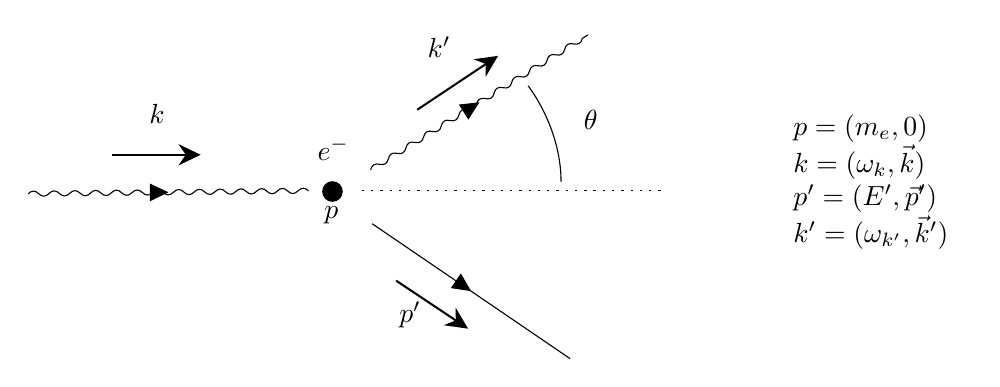
\begin{tikzpicture}[x=0.75pt,y=0.75pt,yscale=-1,xscale=1]
%uncomment if require: \path (0,300); %set diagram left start at 0, and has height of 300

%Straight Lines [id:da47004371895046315] 
\draw    (94,144.56) .. controls (95.65,142.87) and (97.31,142.85) .. (99,144.5) .. controls (100.68,146.15) and (102.35,146.13) .. (104,144.45) .. controls (105.65,142.77) and (107.32,142.75) .. (109,144.4) .. controls (110.69,146.05) and (112.35,146.03) .. (114,144.34) .. controls (115.65,142.66) and (117.32,142.64) .. (119,144.29) .. controls (120.69,145.94) and (122.35,145.92) .. (124,144.23) .. controls (125.65,142.55) and (127.32,142.53) .. (129,144.18) .. controls (130.68,145.83) and (132.35,145.81) .. (134,144.13) .. controls (135.65,142.44) and (137.31,142.42) .. (139,144.07) .. controls (140.68,145.72) and (142.35,145.7) .. (144,144.02) .. controls (145.65,142.34) and (147.32,142.32) .. (149,143.97) .. controls (150.69,145.62) and (152.35,145.6) .. (154,143.91) .. controls (155.65,142.23) and (157.32,142.21) .. (159,143.86) .. controls (160.68,145.51) and (162.35,145.49) .. (164,143.81) .. controls (165.65,142.12) and (167.31,142.1) .. (169,143.75) .. controls (170.68,145.4) and (172.35,145.38) .. (174,143.7) .. controls (175.65,142.02) and (177.32,142) .. (179,143.65) .. controls (180.69,145.3) and (182.35,145.28) .. (183.99,143.59) .. controls (185.64,141.91) and (187.31,141.89) .. (188.99,143.54) .. controls (190.67,145.19) and (192.34,145.17) .. (193.99,143.49) .. controls (195.64,141.8) and (197.3,141.78) .. (198.99,143.43) .. controls (200.67,145.08) and (202.34,145.06) .. (203.99,143.38) .. controls (205.64,141.7) and (207.31,141.68) .. (208.99,143.33) .. controls (210.68,144.98) and (212.34,144.96) .. (213.99,143.27) .. controls (215.64,141.59) and (217.31,141.57) .. (218.99,143.22) .. controls (220.67,144.87) and (222.34,144.85) .. (223.99,143.17) .. controls (225.64,141.48) and (227.3,141.46) .. (228.99,143.11) -- (229.06,143.11) -- (229.06,143.11) ;
\draw [shift={(161.53,143.83)}, rotate = 539.39] [fill={rgb, 255:red, 0; green, 0; blue, 0 }  ][line width=0.08]  [draw opacity=0] (8.93,-4.29) -- (0,0) -- (8.93,4.29) -- cycle    ;
%Flowchart: Connector [id:dp08357812112166041] 
\draw  [fill={rgb, 255:red, 0; green, 0; blue, 0 }  ,fill opacity=1 ] (235.89,143.47) .. controls (235.89,146.06) and (237.99,148.17) .. (240.58,148.17) .. controls (243.18,148.17) and (245.28,146.06) .. (245.28,143.47) .. controls (245.28,140.88) and (243.18,138.78) .. (240.58,138.78) .. controls (237.99,138.78) and (235.89,140.88) .. (235.89,143.47) -- cycle ;
%Straight Lines [id:da8179679192746647] 
\draw    (259,133) .. controls (259.54,130.71) and (260.96,129.83) .. (263.25,130.36) .. controls (265.54,130.9) and (266.96,130.02) .. (267.5,127.73) .. controls (268.03,125.44) and (269.45,124.56) .. (271.74,125.09) .. controls (274.03,125.62) and (275.45,124.74) .. (275.99,122.45) .. controls (276.53,120.16) and (277.95,119.28) .. (280.24,119.82) .. controls (282.53,120.35) and (283.95,119.47) .. (284.49,117.18) .. controls (285.03,114.89) and (286.45,114.01) .. (288.74,114.54) .. controls (291.03,115.08) and (292.45,114.2) .. (292.99,111.91) .. controls (293.52,109.62) and (294.94,108.74) .. (297.23,109.27) .. controls (299.52,109.8) and (300.94,108.92) .. (301.48,106.63) .. controls (302.02,104.34) and (303.44,103.46) .. (305.73,104) .. controls (308.02,104.53) and (309.44,103.65) .. (309.98,101.36) .. controls (310.52,99.07) and (311.94,98.19) .. (314.23,98.72) .. controls (316.52,99.25) and (317.94,98.37) .. (318.47,96.08) .. controls (319.01,93.79) and (320.43,92.91) .. (322.72,93.45) .. controls (325.01,93.98) and (326.43,93.1) .. (326.97,90.81) .. controls (327.51,88.52) and (328.93,87.64) .. (331.22,88.17) .. controls (333.51,88.71) and (334.93,87.83) .. (335.47,85.54) .. controls (336.01,83.25) and (337.43,82.37) .. (339.72,82.9) .. controls (342.01,83.43) and (343.43,82.55) .. (343.96,80.26) .. controls (344.5,77.97) and (345.92,77.09) .. (348.21,77.63) .. controls (350.5,78.16) and (351.92,77.28) .. (352.46,74.99) .. controls (353,72.7) and (354.42,71.82) .. (356.71,72.35) .. controls (359,72.89) and (360.42,72.01) .. (360.96,69.72) -- (363.72,68) -- (363.72,68) ;
\draw [shift={(311.36,100.5)}, rotate = 508.17] [fill={rgb, 255:red, 0; green, 0; blue, 0 }  ][line width=0.08]  [draw opacity=0] (8.93,-4.29) -- (0,0) -- (8.93,4.29) -- cycle    ;
%Straight Lines [id:da15056850292634993] 
\draw  [dash pattern={on 0.84pt off 2.51pt}]  (254.67,143.11) -- (399.83,143.11) ;
%Curve Lines [id:da5581541176414646] 
\draw    (334.83,92.56) .. controls (343.5,104.11) and (350.72,121.44) .. (350.72,138.78) ;
%Straight Lines [id:da0395906445138241] 
\draw    (259.72,159) -- (355.06,224) ;
\draw [shift={(307.39,191.5)}, rotate = 214.29] [fill={rgb, 255:red, 0; green, 0; blue, 0 }  ][line width=0.08]  [draw opacity=0] (8.93,-4.29) -- (0,0) -- (8.93,4.29) -- cycle    ;
%Straight Lines [id:da452390952963887] 
\draw [line width=0.75]    (134.44,125.78) -- (174.06,125.78) ;
\draw [shift={(177.06,125.78)}, rotate = 180] [fill={rgb, 255:red, 0; green, 0; blue, 0 }  ][line width=0.08]  [draw opacity=0] (10.72,-5.15) -- (0,0) -- (10.72,5.15) -- (7.12,0) -- cycle    ;
%Straight Lines [id:da857484560177197] 
\draw [line width=0.75]    (281.39,104.11) -- (317.89,79.78) ;
\draw [shift={(320.39,78.11)}, rotate = 506.31] [fill={rgb, 255:red, 0; green, 0; blue, 0 }  ][line width=0.08]  [draw opacity=0] (10.72,-5.15) -- (0,0) -- (10.72,5.15) -- (7.12,0) -- cycle    ;
%Straight Lines [id:da6224517902495592] 
\draw [line width=0.75]    (271.28,186.44) -- (303.45,207.89) ;
\draw [shift={(305.94,209.56)}, rotate = 213.69] [fill={rgb, 255:red, 0; green, 0; blue, 0 }  ][line width=0.08]  [draw opacity=0] (10.72,-5.15) -- (0,0) -- (10.72,5.15) -- (7.12,0) -- cycle    ;

% Text Node
\draw (365,109) node    {$\theta $};
% Text Node
\draw (156,106) node    {$k$};
% Text Node
\draw (292,74) node    {$k'$};
% Text Node
\draw (278,203) node    {$p'$};
% Text Node
\draw (241,123) node    {$e^{-}$};
% Text Node
\draw (240,155) node    {$p$};
%Text Node
\draw (500,139) node    {$ \begin{array}{l}
p=( m_{e} ,0)\\
k=( \omega _{k} ,\vec{k})\\
p'=( E',\vec{p} ')\\
k'=( \omega _{k'} ,\vec{k} ')
\end{array}$};


\end{tikzpicture}
\end{figure}

We will express the cross section in terms of $\omega$ and $\theta$. We can find $\omega'$, the energy of the final photon, using the following trick:
\begin{align*}
m^2&=(p')^2=(p+k-k')^2=p^2+2p\cdot(k-k')-2k\cdot k'\\
&=m^2+2m(\omega_k-\omega_{k'})-2\omega_k\omega_{k'}(1-\cos\theta)
\end{align*}
hence, we obtain Compton's formula for the shift in the photon wavelength:
\[\Delta\lambda=\left(\frac1{\omega_{k'}}-\frac1{\omega_{k}}\right)=\frac{1-\cos\theta}{m}\]
For our purposes, however, is more useful to solve for $\omega_{k'}$:
\begin{equation}\label{eqn:QED-compton-energies-lab}
\omega_{k'}=\frac{\omega_k}{1+\frac{\omega_{k}}m(1-\cos\theta)}
\end{equation}

The unpolarized amplitude in the Lab frame is
\begin{align*}
|\bar{\mathcal M}|_{\textup{LAB}}^2&=2q^4\left[\left(\frac{\omega_{k'}}{\omega_k}+\frac{\omega_k}{\omega_{k'}}\right)+2m\left(\frac1{\omega_k}-\frac1{\omega_{k'}}\right)+m^2\left(\frac1{\omega_k}-\frac1{\omega_{k'}}\right)^2\right]\\
&=2q^4\left[\left(\frac{\omega_{k'}}{\omega_k}+\frac{\omega_k}{\omega_{k'}}\right)-\sin^2\theta\right]
\end{align*}

The covariant flux factor reads
\[I_{\textup{LAB}}=[(p\cdot k)^2-m_e^2m_\gamma^2]^{1/2}=|p\cdot k|=m_e\omega_k\]
The 2-body phase space
\begin{align*}
\int\de\Phi_{(2)}&=\int \frac{\de^3k'}{(2\pi)^32\omega_{k'}}\frac{\de^3p'}{(2\pi)^32E'}(2\pi)^4\delta^4(k'+p'-k-p)
=\int\frac{\omega^2_{k'}\de\omega_{k'}\de\Omega}{(2\pi)^2}\frac{1}{4\omega_{k'}E'}\delta(\omega_{k'}+E'-\omega_k-m)\\
&=\int\frac{\omega^2_{k'}\de\omega_{k'}\de\Omega}{(2\pi)^2}\frac{1}{4\omega_{k'}E'}\frac{\delta(\omega_{k'}-|\vec k'|)}{\left|\frac{\partial(\omega_{k'}+E'-\omega_k-m)}{\partial|k'|}\right|}_{\omega_{k'}=|\vec k'|}
=\int\de\Omega\frac{|\vec k'|^2}{16\pi^2\omega_{k'}E'}\left|\frac{\partial(\omega_{k'}+E')}{\partial|k'|}\right|^{-1}_{\omega_{k'}=|\vec k'|}
\end{align*}
where 
\[E'=\left(m^2+(\vec k-\vec k')^2\right)^{1/2}
=\left[m^2+\omega_k^2+\omega_{k'}^2-2\omega_{k'}\omega_k\cos\theta\right]^{1/2}\]
\[\frac{\partial E'}{\partial|k'|}=\frac{\omega_{k'}-\omega_k\cos\theta}{E'}\]
and
\todo{Controlla l'ultimo passaggio}

\[\left|\frac{\partial(\omega_{k'}+E')}{\partial|k'|}\right|_{\omega_{k'}=|\vec k'|}
=\left|1+\frac{\omega_{k'}-\omega_k\cos\theta}{E'}\right|
=\frac{m\omega_k}{E'\omega_{k'}}
\]
So the unpolarized cross section is 
\begin{align*}
\left(\frac{\de\bar\sigma}{\de\Omega}\right)_{\textup{LAB}}&=
\frac{\overline{|\mathcal M|}_{\textup{LAB}}^2}{4I_{\textup{LAB}}}\frac{\de\Phi_{(2)}}{\de\Omega}
=\frac1{64\pi^2}\frac{|\vec k'|^2}{I_{\textup{LAB}}\omega_{k'}E'}\left|\frac{\partial(\omega_{k'}+E')}{\partial|k'|}\right|^{-1}\overline{|\mathcal M|}_{\textup{LAB}}^2\\
&=\frac{q^4}{32\pi^2}\frac1{m^2}\left(\frac{\omega_{k'}}{\omega_k}\right)^2\left(\frac{\omega_{k'}}{\omega_k}+\frac{\omega_k}{\omega_{k'}}-\sin^2\theta\right)\\
&=\frac{\alpha^2}{2}\frac1{m^2}\left(\frac{\omega_{k'}}{\omega_k}\right)^2\left(\frac{\omega_{k'}}{\omega_k}+\frac{\omega_k}{\omega_{k'}}-\sin^2\theta\right)
\end{align*}
where $\omega_{k'}/\omega_{k}$ is given by \eqref{eqn:QED-compton-energies-lab} and in the last step we used $\alpha=e^2/(4\pi)$. Writing $\de\Omega=(2\pi)\de\cos\theta$ we obtain
\begin{align}\label{eqn:Klein-Nishina}
\left(\frac{\de\bar\sigma}{\de\cos\theta}\right)_{\textup{LAB}}&=
\frac{\pi\alpha^2}{m^2}\left(\frac{\omega_{k'}}{\omega_k}\right)^2\left(\frac{\omega_{k'}}{\omega_k}+\frac{\omega_k}{\omega_{k'}}-\sin^2\theta\right)
\end{align}

This is the (spin-averaged) \emph{Klein-Nishina formula}.
In the low energy limit $\omega_k\ll m$, from \eqref{eqn:QED-compton-energies-lab} we have $\omega_{k'}\approx\omega_{k}$, i.e. the kinetic energy of the recoil electron is negligible, and Eq.\eqref{eqn:Klein-Nishina} reduces to the familiar Thomson cross-section for scattering of classical electromagnetic radiation by a free electron:

\begin{align*}
\left(\frac{\de\bar\sigma}{\de\cos\theta}\right)_{\textup{LAB}}&\overset{\omega_k\ll m}{=}
\frac{\pi\alpha^2}{m^2}\left(1+\cos^2\theta\right)
\quad\rightarrow\quad
(\bar\sigma)_{\textup{LAB}}=\frac{8\pi\alpha^2}{3m^2}\equiv\frac83\pi r_e^2
\end{align*}

We have calculated the full relativistic corrections for the Thomson formula.

\subsection{C.o.M. frame - High energy photon}
To analyze the high-energy behaviour of the Compton scattering cross section, it is easiest to work in the center-of-mass frame.

\begin{figure}[H]
\centering


\tikzset{every picture/.style={line width=0.75pt}} %set default line width to 0.75pt        

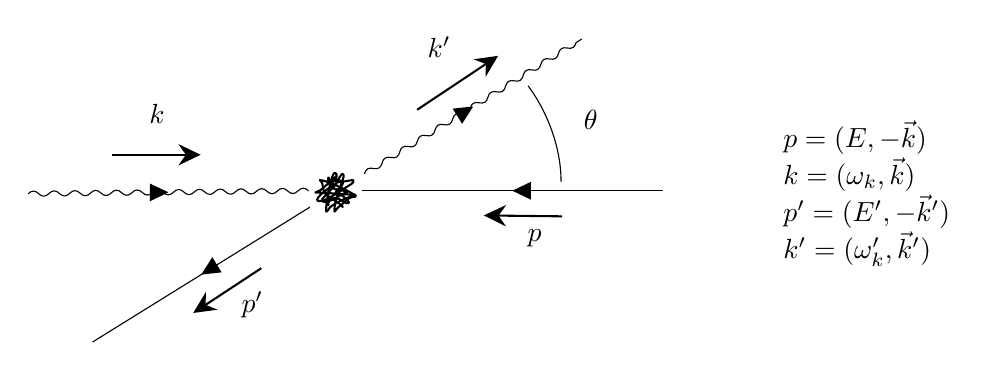
\begin{tikzpicture}[x=0.75pt,y=0.75pt,yscale=-1,xscale=1]
%uncomment if require: \path (0,300); %set diagram left start at 0, and has height of 300

%Straight Lines [id:da2201162405089543] 
\draw    (94,144.56) .. controls (95.65,142.87) and (97.31,142.85) .. (99,144.5) .. controls (100.68,146.15) and (102.35,146.13) .. (104,144.45) .. controls (105.65,142.77) and (107.32,142.75) .. (109,144.4) .. controls (110.69,146.05) and (112.35,146.03) .. (114,144.34) .. controls (115.65,142.66) and (117.32,142.64) .. (119,144.29) .. controls (120.69,145.94) and (122.35,145.92) .. (124,144.23) .. controls (125.65,142.55) and (127.32,142.53) .. (129,144.18) .. controls (130.68,145.83) and (132.35,145.81) .. (134,144.13) .. controls (135.65,142.44) and (137.31,142.42) .. (139,144.07) .. controls (140.68,145.72) and (142.35,145.7) .. (144,144.02) .. controls (145.65,142.34) and (147.32,142.32) .. (149,143.97) .. controls (150.69,145.62) and (152.35,145.6) .. (154,143.91) .. controls (155.65,142.23) and (157.32,142.21) .. (159,143.86) .. controls (160.68,145.51) and (162.35,145.49) .. (164,143.81) .. controls (165.65,142.12) and (167.31,142.1) .. (169,143.75) .. controls (170.68,145.4) and (172.35,145.38) .. (174,143.7) .. controls (175.65,142.02) and (177.32,142) .. (179,143.65) .. controls (180.69,145.3) and (182.35,145.28) .. (183.99,143.59) .. controls (185.64,141.91) and (187.31,141.89) .. (188.99,143.54) .. controls (190.67,145.19) and (192.34,145.17) .. (193.99,143.49) .. controls (195.64,141.8) and (197.3,141.78) .. (198.99,143.43) .. controls (200.67,145.08) and (202.34,145.06) .. (203.99,143.38) .. controls (205.64,141.7) and (207.31,141.68) .. (208.99,143.33) .. controls (210.68,144.98) and (212.34,144.96) .. (213.99,143.27) .. controls (215.64,141.59) and (217.31,141.57) .. (218.99,143.22) .. controls (220.67,144.87) and (222.34,144.85) .. (223.99,143.17) .. controls (225.64,141.48) and (227.3,141.46) .. (228.99,143.11) -- (229.06,143.11) -- (229.06,143.11) ;
\draw [shift={(161.53,143.83)}, rotate = 539.39] [fill={rgb, 255:red, 0; green, 0; blue, 0 }  ][line width=0.08]  [draw opacity=0] (8.93,-4.29) -- (0,0) -- (8.93,4.29) -- cycle    ;
%Straight Lines [id:da8440776864610582] 
\draw    (256,135) .. controls (256.54,132.71) and (257.96,131.83) .. (260.25,132.36) .. controls (262.54,132.9) and (263.96,132.02) .. (264.5,129.73) .. controls (265.03,127.44) and (266.45,126.56) .. (268.74,127.09) .. controls (271.03,127.62) and (272.45,126.74) .. (272.99,124.45) .. controls (273.53,122.16) and (274.95,121.28) .. (277.24,121.82) .. controls (279.53,122.35) and (280.95,121.47) .. (281.49,119.18) .. controls (282.03,116.89) and (283.45,116.01) .. (285.74,116.54) .. controls (288.03,117.08) and (289.45,116.2) .. (289.99,113.91) .. controls (290.52,111.62) and (291.94,110.74) .. (294.23,111.27) .. controls (296.52,111.8) and (297.94,110.92) .. (298.48,108.63) .. controls (299.02,106.34) and (300.44,105.46) .. (302.73,106) .. controls (305.02,106.53) and (306.44,105.65) .. (306.98,103.36) .. controls (307.52,101.07) and (308.94,100.19) .. (311.23,100.72) .. controls (313.52,101.25) and (314.94,100.37) .. (315.47,98.08) .. controls (316.01,95.79) and (317.43,94.91) .. (319.72,95.45) .. controls (322.01,95.98) and (323.43,95.1) .. (323.97,92.81) .. controls (324.51,90.52) and (325.93,89.64) .. (328.22,90.17) .. controls (330.51,90.71) and (331.93,89.83) .. (332.47,87.54) .. controls (333.01,85.25) and (334.43,84.37) .. (336.72,84.9) .. controls (339.01,85.43) and (340.43,84.55) .. (340.96,82.26) .. controls (341.5,79.97) and (342.92,79.09) .. (345.21,79.63) .. controls (347.5,80.16) and (348.92,79.28) .. (349.46,76.99) .. controls (350,74.7) and (351.42,73.82) .. (353.71,74.35) .. controls (356,74.89) and (357.42,74.01) .. (357.96,71.72) -- (360.72,70) -- (360.72,70) ;
\draw [shift={(308.36,102.5)}, rotate = 508.17] [fill={rgb, 255:red, 0; green, 0; blue, 0 }  ][line width=0.08]  [draw opacity=0] (8.93,-4.29) -- (0,0) -- (8.93,4.29) -- cycle    ;
%Straight Lines [id:da09307133911969756] 
\draw    (254.67,143.11) -- (399.83,143.11) ;
\draw [shift={(327.25,143.11)}, rotate = 0] [fill={rgb, 255:red, 0; green, 0; blue, 0 }  ][line width=0.08]  [draw opacity=0] (8.93,-4.29) -- (0,0) -- (8.93,4.29) -- cycle    ;
%Curve Lines [id:da33812291607616296] 
\draw    (334.83,92.56) .. controls (343.5,104.11) and (350.72,121.44) .. (350.72,138.78) ;
%Straight Lines [id:da5774490131113152] 
\draw [line width=0.75]    (134.44,125.78) -- (174.06,125.78) ;
\draw [shift={(177.06,125.78)}, rotate = 180] [fill={rgb, 255:red, 0; green, 0; blue, 0 }  ][line width=0.08]  [draw opacity=0] (10.72,-5.15) -- (0,0) -- (10.72,5.15) -- (7.12,0) -- cycle    ;
%Straight Lines [id:da24269378260147034] 
\draw [line width=0.75]    (281.39,104.11) -- (317.89,79.78) ;
\draw [shift={(320.39,78.11)}, rotate = 506.31] [fill={rgb, 255:red, 0; green, 0; blue, 0 }  ][line width=0.08]  [draw opacity=0] (10.72,-5.15) -- (0,0) -- (10.72,5.15) -- (7.12,0) -- cycle    ;
%Straight Lines [id:da3757335905736008] 
\draw [line width=0.75]    (206.28,180.44) -- (176.01,200.35) ;
\draw [shift={(173.5,202)}, rotate = 326.66999999999996] [fill={rgb, 255:red, 0; green, 0; blue, 0 }  ][line width=0.08]  [draw opacity=0] (10.72,-5.15) -- (0,0) -- (10.72,5.15) -- (7.12,0) -- cycle    ;
%Straight Lines [id:da04091628549293125] 
\draw    (125,216) -- (229.72,151) ;
\draw [shift={(177.36,183.5)}, rotate = 328.17] [fill={rgb, 255:red, 0; green, 0; blue, 0 }  ][line width=0.08]  [draw opacity=0] (8.93,-4.29) -- (0,0) -- (8.93,4.29) -- cycle    ;
%Straight Lines [id:da587248071756918] 
\draw [line width=0.75]    (351.28,155.44) -- (316.5,155.04) ;
\draw [shift={(313.5,155)}, rotate = 360.66999999999996] [fill={rgb, 255:red, 0; green, 0; blue, 0 }  ][line width=0.08]  [draw opacity=0] (10.72,-5.15) -- (0,0) -- (10.72,5.15) -- (7.12,0) -- cycle    ;
%Shape: Free Drawing [id:dp672077562881797] 
\draw  [color={rgb, 255:red, 0; green, 0; blue, 0 }  ][line width=0.75] [line join = round][line cap = round] (238.5,139) .. controls (238.5,134.42) and (238.79,137.16) .. (239.5,140) .. controls (239.61,140.46) and (240.17,139.33) .. (240.5,139) .. controls (241.52,137.98) and (244.74,137.49) .. (245.5,139) .. controls (246.37,140.74) and (240.56,144) .. (242.5,144) .. controls (244.25,144) and (249.12,148.69) .. (248.5,149) .. controls (246.85,149.82) and (245.13,147.33) .. (243.5,147) .. controls (242.19,146.74) and (240.69,146.4) .. (239.5,147) .. controls (238.56,147.47) and (238.5,151.05) .. (238.5,150) .. controls (238.5,145.09) and (238.54,139.96) .. (241.5,137) .. controls (241.83,136.67) and (242.5,136) .. (242.5,136) .. controls (242.5,136) and (235.39,142.55) .. (234.5,143) .. controls (233.83,143.33) and (231.75,144) .. (232.5,144) .. controls (238.77,144) and (245.98,145) .. (251.5,145) .. controls (253.3,145) and (248.11,146.2) .. (246.5,147) .. controls (244.9,147.8) and (240.81,149.69) .. (239.5,151) .. controls (238.83,151.67) and (237.73,153.91) .. (237.5,153) .. controls (237.11,151.43) and (240.32,130.65) .. (242.5,135) .. controls (243.1,136.19) and (241.39,138.26) .. (242.5,139) .. controls (243.03,139.35) and (250.31,137.81) .. (250.5,138) .. controls (251.19,138.69) and (249.76,139.87) .. (249.5,140) .. controls (247.14,141.18) and (236.38,149.44) .. (233.5,148) .. controls (231.39,146.95) and (240.55,140) .. (242.5,140) ;
%Shape: Free Drawing [id:dp3629185907562005] 
\draw  [color={rgb, 255:red, 0; green, 0; blue, 0 }  ][line width=0.75] [line join = round][line cap = round] (245.5,151) .. controls (245.5,149.77) and (238.43,145.93) .. (237.5,145) .. controls (235.85,143.35) and (236.16,140.97) .. (235.5,139) .. controls (235.35,138.55) and (234.03,138) .. (234.5,138) .. controls (237.62,138) and (245.48,141.99) .. (247.5,143) .. controls (248.99,143.75) and (253.17,146) .. (251.5,146) .. controls (247.23,146) and (245.77,149.87) .. (243.5,151) .. controls (242.66,151.42) and (241.5,153.94) .. (241.5,153) .. controls (241.5,147.47) and (243.79,143.12) .. (245.5,138) .. controls (245.82,137.05) and (246.39,135.45) .. (245.5,135) .. controls (244.77,134.63) and (241.54,140.96) .. (241.5,141) .. controls (240.88,141.62) and (234.76,147.26) .. (235.5,148) .. controls (237.89,150.39) and (245.38,144) .. (247.5,144) .. controls (248.25,144) and (246.21,143.24) .. (245.5,143) .. controls (243.55,142.35) and (241.34,142.84) .. (239.5,141) ;

% Text Node
\draw (365,109) node    {$\theta $};
% Text Node
\draw (156,106) node    {$k$};
% Text Node
\draw (292,74) node    {$k'$};
% Text Node
\draw (202,198) node    {$p'$};
% Text Node
\draw (338,166) node    {$p$};
% Text Node
\draw (498,145) node    {$ \begin{array}{l}
p=( E,-\vec{k})\\
k=( \omega _{k} ,\vec{k})\\
p'=( E',-\vec{k} ')\\
k'=( \omega _{k} ',\vec{k} ')
\end{array}$};


\end{tikzpicture}
\end{figure}

The kinematics of the reaction in the high energy limit ($m\approx0$) looks like
\begin{align*}
E&=\sqrt{\vec k^2+m^2}\approx|\vec k|=\omega_k\\
E'&=\sqrt{\vec k'^2+m^2}\approx|\vec k'|=\omega_{k'}
\end{align*}
\begin{align*}
p\cdot k&=\omega_k^2+|\vec k|^2=2\omega_k^2\\
p\cdot p'&=\omega_k\omega_{k'}-\vec k\vec k'=\omega_k\omega_{k'}-|\vec k||\vec k'|\cos\theta=\omega_k\omega_{k'}(1-\cos\theta)\\
k'\cdot p&=\omega_k\omega_{k'}+\vec k\vec k'=\omega_k\omega_{k'}+|\vec k||\vec k'|\cos\theta=\omega_k\omega_{k'}(1+\cos\theta)
\end{align*}
We also have
\begin{align*}
s&=(p+k)^2=(E+\omega_k)^2=4\omega_k^2 \quad\rightarrow\quad \omega_k=\frac{\sqrt s}{2}\\
&=(p'+k')^2=(E'+\omega_{k'})^2=4\omega_{k'}^2 \quad\rightarrow\quad \omega_{k'}=\frac{\sqrt s}{2}
\end{align*}
So Mandelstam variables in high energy limit ($m=0$) take the form
\begin{align*}
s&=(p+k)^2=(p'+k')^2\approx2p\cdot k=4\omega_k^2\\
t&=(p'-p)^2=(k'-k)^2\approx -2p\cdot p'=-2\omega_k^2(1-\cos\theta)\\
u&=(k'-p)^2=(p'-k)^2\approx-2k'\cdot p=-2\omega_k^2(1+\cos\theta)
\end{align*}














\onlyinmainfile{\begin{comment}} %Lascio il codice qui per vedere come hai fatto te le cose 

\section{Sezioni di esempio}
Consider the case in which the initial state is a single particle and the final state is given by n particles. We are therefore considering a decay process. Assume for the moment that particles are indistinguishable.

\begin{center}
\tikzset{every picture/.style={line width=0.75pt}} %set default line width to 0.75pt        
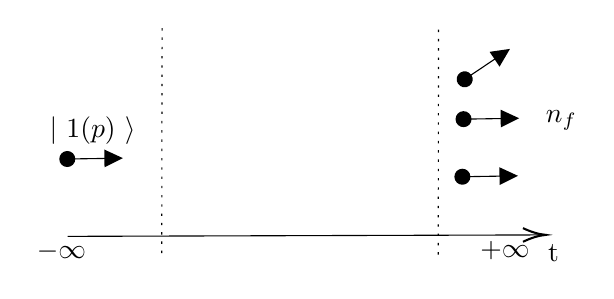
\begin{tikzpicture}[x=0.75pt,y=0.75pt,yscale=-1,xscale=1]
%uncomment if require: \path (0,194); %set diagram left start at 0, and has height of 194

%Straight Lines [id:da28910037002363764] 
\draw    (205.27,107.68) -- (433.59,106.98) ;
\draw [shift={(435.59,106.97)}, rotate = 539.8199999999999] [color={rgb, 255:red, 0; green, 0; blue, 0 }  ][line width=0.75]    (10.93,-3.29) .. controls (6.95,-1.4) and (3.31,-0.3) .. (0,0) .. controls (3.31,0.3) and (6.95,1.4) .. (10.93,3.29)   ;
%Straight Lines [id:da7985070919800723] 
\draw  [dash pattern={on 0.84pt off 2.51pt}]  (250.78,7.4) -- (250.61,116.64) ;
%Straight Lines [id:da47959589803581304] 
\draw  [dash pattern={on 0.84pt off 2.51pt}]  (383.98,8.11) -- (383.81,117.35) ;
%Straight Lines [id:da17940445023321017] 
\draw    (205.1,70.41) -- (228.91,70.04) ;
\draw [shift={(231.91,69.99)}, rotate = 539.0899999999999] [fill={rgb, 255:red, 0; green, 0; blue, 0 }  ][line width=0.08]  [draw opacity=0] (8.93,-4.29) -- (0,0) -- (8.93,4.29) -- cycle    ;
\draw [shift={(205.1,70.41)}, rotate = 359.09] [color={rgb, 255:red, 0; green, 0; blue, 0 }  ][fill={rgb, 255:red, 0; green, 0; blue, 0 }  ][line width=0.75]      (0, 0) circle [x radius= 3.35, y radius= 3.35]   ;
%Straight Lines [id:da9397044962896224] 
\draw    (396.57,32.01) -- (415.9,19.03) ;
\draw [shift={(418.39,17.36)}, rotate = 506.11] [fill={rgb, 255:red, 0; green, 0; blue, 0 }  ][line width=0.08]  [draw opacity=0] (8.93,-4.29) -- (0,0) -- (8.93,4.29) -- cycle    ;
\draw [shift={(396.57,32.01)}, rotate = 326.11] [color={rgb, 255:red, 0; green, 0; blue, 0 }  ][fill={rgb, 255:red, 0; green, 0; blue, 0 }  ][line width=0.75]      (0, 0) circle [x radius= 3.35, y radius= 3.35]   ;
%Straight Lines [id:da4306245684857515] 
\draw    (395.46,78.95) -- (419.27,78.57) ;
\draw [shift={(422.27,78.52)}, rotate = 539.0899999999999] [fill={rgb, 255:red, 0; green, 0; blue, 0 }  ][line width=0.08]  [draw opacity=0] (8.93,-4.29) -- (0,0) -- (8.93,4.29) -- cycle    ;
\draw [shift={(395.46,78.95)}, rotate = 359.09] [color={rgb, 255:red, 0; green, 0; blue, 0 }  ][fill={rgb, 255:red, 0; green, 0; blue, 0 }  ][line width=0.75]      (0, 0) circle [x radius= 3.35, y radius= 3.35]   ;
%Straight Lines [id:da8816879387506134] 
\draw    (396.02,51.21) -- (419.83,50.83) ;
\draw [shift={(422.83,50.78)}, rotate = 539.0899999999999] [fill={rgb, 255:red, 0; green, 0; blue, 0 }  ][line width=0.08]  [draw opacity=0] (8.93,-4.29) -- (0,0) -- (8.93,4.29) -- cycle    ;
\draw [shift={(396.02,51.21)}, rotate = 359.09] [color={rgb, 255:red, 0; green, 0; blue, 0 }  ][fill={rgb, 255:red, 0; green, 0; blue, 0 }  ][line width=0.75]      (0, 0) circle [x radius= 3.35, y radius= 3.35]   ;


% Text Node
\draw (443.19,51.92) node    {$n_{f}$};
% Text Node
\draw (217.31,56.9) node    {$|\ 1( p) \ \rangle $};
% Text Node
\draw (439.31,115.93) node   [align=left] {t};
% Text Node
\draw (202.32,115.22) node    {$-\infty $};
% Text Node
\draw (416,114.51) node    {$+\infty $};

\end{tikzpicture}
\end{center}

The rules of quantum mechanics tell us that the probability for this process is obtained by taking the squared modulus of the amplitude and summing over all possible final states
\[
\begin{split}
\abs{S_{fi}^{CN}}^2	& = \abs{(2 \pi)^4 \delta^4 (p - p')M_{fi}^{CN}}^2 \\
				& = (2 \pi)^4 \delta^4 (p - p') (VT) \abs{M_{fi}^{CN}}^2 \\
				& = (2 \pi)^4 \delta^4 (p - p')(VT) \frac{1}{2 \omega_in V}
					\prod_{l=1}^{n_f} \biggl( \frac{1}{2 \omega_l V} \biggr) \abs{\mathM_{fi}}^2
\end{split}
\]
\textbf{Note:} $\bigl( \delta^4 (p - p') \bigr)^2 = \delta^4 (p - p') \delta^4 (p - p') = \delta^4 (p - p') \delta^4(0) = \delta^4 (p - p') \frac{VT}{(2 \pi)^4}$\\
We use the final space and time in order to remove divergent terms during calculation\\ \\
We must now sum this expression over all final states. Since we are working in a finite volume V, this is the sum over the possible discrete values of the momenta of the final particles .\\
Since $p_i = (2 \pi/L) n_i$, we have $dn_i = (L/2\pi) \de p_i$ and $\de^3 n_i = (V/(2 \pi)^3) \de^3 p$ where $\de^3 n_i$ is the infinitesimal phase space related to a final state in which the i-th particle has momentum between $p_i$ and $p_i + \de p_i$\\
Let $\de \omega$ be the probability for a decay in which in the final state the i-th particle has momentum between $p_i$ and $p_i \de p_i$
\[
\de \omega = \abs{S_{fi}^{SN}}^2 \prod_{l=1}^{n_f} \biggl( \frac{V\de^3 p_l}{(2 \pi)^3} \biggr)
\]
This is the probability that the decay takes place in any time between $-T/2$ and $T/2$. We are more interested in the differential decay rate $\de \Gamma_{fi}$, which is the decay probability per unit of time:
\[
\de \Gamma_{fi} = \frac{\de \omega}{T} = (2 \pi)^4 \delta^4 (p_i - p_f) \frac{\abs{\mathM_{fi}}^2}{2 \omega_{p_{in}}}
	\prod_{l=1}^{n_f} \frac{\de^3 p_l}{(2 \pi)^3 2 \omega_l}
\]
\textbf{Notes:}
\begin{enumerate}
\item $\de \Gamma_{fi}$ = differential decay rate
\item $p_f$ = sum over final momenta
\item $\omega_{p_{in}}$ = initial energy
\item $\abs{\mathM_{fi}}^2$ = Feynman amplitude of the process (depends on final momenta $p_i$)
\end{enumerate}
It is useful to define the \textbf{(differential) n-body phase space} as
\[
\de \Phi_{(n_f)} = (2 \pi)^4 \delta^4 (p_i - p_f) \prod_{l=1}^{n_f} \frac{\de^3 p_l}{(2 \pi)^3 2 \omega_l}
\]
Therefore the differential decay rate can be written as
\[
\de \Gamma_{fi} = \frac{1}{2 \omega_{p_{in}}} \abs{\mathM_{fi}}^2 \de \Phi_{(n_f)}
\]
The decay rate is defined as
\[
\Gamma_{fi} = \int \de \Gamma_{fi}
\quad
\to \textup{integration over all possible final momenta}
\]
and its meaning is $\Gamma \equiv$ trans. probability $\times$ unit of time $\times$ \ init. particle\\
Notice that if n of the final particles are identical, configurations that differ by a permutation are not distinct and therefore the phase space is reduced by a factor $1/h!$\\
If we have a system of N(0) particles, the time evolution of the number of particles N(t) is
\[
\frac{\de N}{\de t} = - \Gamma N
\quad \so \quad
N(t) = N(0) e^{-\Gamma t}
\]
Notice that decay rate is not invariant
\[
\bigl[ \Gamma \bigr] = \bigl[ E \bigr] = \frac{1}{T}
\qquad
\textup{(in natural units)}
\]
If we define the \textbf{lifetime} as $\tau = 1/\Gamma \so N(t) = N(0) \exp(-t/\tau)$ this changes under Lorentz tfm. If we consider two reference frames o and o'
\[
\Gamma' = \frac{\Gamma}{\gamma} < \Gamma
\qquad
\tau' = \gamma \tau > \tau
\]
$\gamma = (1 - v)^{-1/2}$, where v is the speed of o' in o in natural units, $\gamma > 1$. Therefore a article in a moving frame has a longer lifetime then in the rest frame\\ \\
\begin{example}[muon lifetime]
For a muon in the rest frame $\tau_{\mu}^{RF} = 2.2 \times 10^{-6} s$, but if we observe it in the lab frame \\
$\tau_{\mu}^{LAB} = \gamma \tau_{\mu}^{RF} \simeq 2 \times 10^{-5} s$ since $E_{\mu}$ = 1 GeV, $m_{\mu}$ = 0.1 GeV \\
$\so \gamma = E_{\mu} / m_{\mu} \simeq 10$ 
\end{example}

\begin{example}[1 $\to$ 2 decay]
Consider the decay of a particle of a mass M into two particles of masses $m_1, m_2$. Since the phase space in Lorentz invariant, we can compute it in the frame that we prefer. We use the rest frame for the initial particle.

\begin{center}
\tikzset{every picture/.style={line width=0.75pt}} %set default line width to 0.75pt        
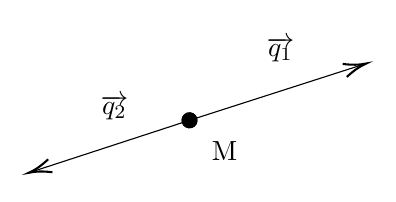
\begin{tikzpicture}[x=0.75pt,y=0.75pt,yscale=-1,xscale=1]
%uncomment if require: \path (0,92); %set diagram left start at 0, and has height of 92
%Straight Lines [id:da19898209267326417] 
\draw    (326.16,55.24) -- (409.47,28.47) ;
\draw [shift={(411.37,27.86)}, rotate = 522.19] [color={rgb, 255:red, 0; green, 0; blue, 0 }  ][line width=0.75]    (10.93,-3.29) .. controls (6.95,-1.4) and (3.31,-0.3) .. (0,0) .. controls (3.31,0.3) and (6.95,1.4) .. (10.93,3.29)   ;
\draw [shift={(326.16,55.24)}, rotate = 342.19] [color={rgb, 255:red, 0; green, 0; blue, 0 }  ][fill={rgb, 255:red, 0; green, 0; blue, 0 }  ][line width=0.75]      (0, 0) circle [x radius= 3.35, y radius= 3.35]   ;
%Straight Lines [id:da5450424757830004] 
\draw    (326.16,55.24) -- (250.59,79.91) ;
\draw [shift={(248.69,80.53)}, rotate = 341.91999999999996] [color={rgb, 255:red, 0; green, 0; blue, 0 }  ][line width=0.75]    (10.93,-3.29) .. controls (6.95,-1.4) and (3.31,-0.3) .. (0,0) .. controls (3.31,0.3) and (6.95,1.4) .. (10.93,3.29)   ;
\draw [shift={(326.16,55.24)}, rotate = 161.92] [color={rgb, 255:red, 0; green, 0; blue, 0 }  ][fill={rgb, 255:red, 0; green, 0; blue, 0 }  ][line width=0.75]      (0, 0) circle [x radius= 3.35, y radius= 3.35]   ;
% Text Node
\draw (343,70) node   [align=left] {M};
% Text Node
\draw (370,21) node    {$\overrightarrow{q_{1}}$};
% Text Node
\draw (290,49) node    {$\overrightarrow{q_{2}}$};
\end{tikzpicture}
\end{center}

We don't impose a priori conservation of momentum since it's imposed by the delta function.
\begin{gather}
p = (M, 0) \qquad
q_1 = (\omega_1, \vec{q_1}) \qquad
q_2 = (\omega_2, q_2) \notag \\
\de \Phi_{(2)} = (2 \pi)^4 \delta^4 \underbrace{(P_i - P_f)}_{= p - q_1 - q_2}
	\frac{\de^3 q_1}{(2 \pi)^3 2 \omega_1} \frac{\de^3 q_2}{(2 \pi)^3 2 \omega_2} \notag
\end{gather}
I have 6 integration parameters, 4 constraint given by $\delta^4$, so I have 2 independent variables. Integrating over $\de^3 q_2$
\[
\de \Phi'_{(2)} = \int \de \Phi_{(2)} = \frac{1}{(2 \pi)^2} \delta(M - \omega_1 - \omega_2) \frac{1}{4 \omega_1 \omega_2} \de^3 q_1
\]
in this way, the condition $\vec{q_2} = \vec{q_1}$ vanish. We have to impose it again when we calculate $\de \Gamma$ (we omit this detail)\\
Usually the 4-th non independent parameter is eliminated by integration over modulus of $q_1$, leaving free 2 parameters for the angles. 
$\de^3 q_1 \to \vec{q_1}^2 \de \abs{\vec{q_2}}\de \Omega_1$.\\ \\
Notice that $M -\omega_1 - \omega_2 = M - \sqrt{\vec{q_1}^2 + m_1^2} - \sqrt{\vec{q_2} + m_2^2}$ and then the $\delta$ implies
\[
\hat{q_1}^2 = \frac{1}{2M} \biggl( M^4 - 2M^2(m_1^2 + m_2^2) + (m_1^2 - m_2^2)^2 \biggr)^{1/2}
\]
$\abs{\vec{q_1}}$ is the only zero of $f(\abs{\hat{q_1}}) = M - \omega_1 - \omega_2$.\\
We also have
\[
\abs{f'(\abs{\hat{q_1}})} = \frac{\partial \omega_1}{\partial \abs{\vec{q_1}}} 
	+ \frac{\partial \omega_2}{\partial \abs{\vec{q_1}}} 
	= \abs{\hat{q_1}} \biggl ( \frac{\omega_1 + \omega_2}{\omega_1 \omega_2} \biggr)
\]
Using
\[
\delta \bigl( f(x) \bigr) = \sum_{x_0 = \textup{zero of f(x)}} \frac{\delta (x - x_0)}{\abs{f'(x_0)}} 
\]
and performing integration over $\de \abs{\vec{q_1}}$ we obtain
\[
\de \Phi''_{(2)} = \int \de \Phi'_{(2)} = \frac{1}{16 \pi^2} \frac{\abs{\hat{q_1}}}{M} \de \Omega_1
\]
Using this result we obtain the $1 \to 2$ decay rate in function of the solid angle (in the rest frame)
\[
\biggl( \frac{\de \Gamma_{RF}}{\de \Omega} \biggr) = \frac{1}{64 \pi^4 M^3}
	\bigl[ M^4 - 2M^2 (m_1^2 + m_2^2) + (m_1 - m_2^2)^2 \bigr]^{1/2} \abs{\mathM_{RF}}^2
\]
In a general frame we can easily obtain an analogous formula, just consider $\de \Gamma = 1/(2 \omega_in) \abs{\mathM_{fi}}^2 \de \Phi_{(nf)}$ in a general frame. remember that $\de I_{(nf)}$ is invariant \\ \\
We have 2 important limit cases:
\begin{enumerate}[label=(\Alph*)]
\item If $m_1 = m_2 = m$ (for example $Z \to e^+ e^-$)
	\begin{gather}
	\abs{\hat{q_1}} = \frac{M}{2} \biggl( 1 - \frac{4 m^2}{M^2} \biggr)^{1/2} \notag \\
	\biggl( \frac{\de \Gamma_{RF}}{\de \Omega} \biggr) = \frac{1}{64 \pi^2 M} \biggl( 1 - \frac{4 m^2}{M^2} \biggl)^{1/2} \abs{\mathM_{fi}}^2 \notag
	\end{gather}
\item If $m_1 = m, m_2 = 0$ (for example $W^{\pm} \to e^{\pm} \stackrel{(-)}{\nu}$)
	\begin{gather}
	\abs{\hat{q_1}} = \frac{M}{2} \biggl( 1 - \frac{4 m^2}{M^2} \biggr)^{1/2} \notag \\
	\biggl( \frac{\de \Gamma_{RF}}{\de \Omega} \biggr) = \frac{1}{64 \pi^2 M} \biggl( 1 - \frac{m^2}{M^2} \biggr)^{1/2} \abs{\mathM_{fi}}^2 \notag
	\end{gather}
\end{enumerate}
\textbf{Notes:} If we have two identical particles in the final state, the calculation of the phase is different
\[
\de \Phi_{(2)}^{\textup{identical}} = \frac{1}{2} \de \Phi_{(2)}^{\textup{distinguishable}}
\]
\end{example}

\section{Cross section ($\leftrightarrow$ scattering process)}

\begin{center}
\tikzset{every picture/.style={line width=0.75pt}} %set default line width to 0.75pt        

\begin{tikzpicture}[x=0.75pt,y=0.75pt,yscale=-1,xscale=1]
%uncomment if require: \path (0,300); %set diagram left start at 0, and has height of 300
%Straight Lines [id:da7420481005024371] 
\draw    (105.3,244) -- (540.3,242.01) ;
\draw [shift={(543.3,242)}, rotate = 539.74] [fill={rgb, 255:red, 0; green, 0; blue, 0 }  ][line width=0.08]  [draw opacity=0] (8.93,-4.29) -- (0,0) -- (8.93,4.29) -- cycle    ;
%Curve Lines [id:da9551272323068936] 
\draw [color={rgb, 255:red, 74; green, 144; blue, 226 }  ,draw opacity=1 ]   (106.07,237.85) .. controls (242.92,240.92) and (179.87,150.21) .. (210.63,127.14) .. controls (229.85,107.92) and (259.83,115.61) .. (357.47,114.84) ;
%Curve Lines [id:da42326511684010204] 
\draw [color={rgb, 255:red, 74; green, 144; blue, 226 }  ,draw opacity=1 ]   (357.47,114.84) .. controls (465.87,114.07) and (332.87,230.16) .. (516.61,237.85) ;
%Straight Lines [id:da05972058678475589] 
\draw    (105.3,197.26) -- (149.47,176.98) ;
\draw [shift={(152.2,175.73)}, rotate = 515.3399999999999] [fill={rgb, 255:red, 0; green, 0; blue, 0 }  ][line width=0.08]  [draw opacity=0] (8.93,-4.29) -- (0,0) -- (8.93,4.29) -- cycle    ;
\draw [shift={(105.3,197.26)}, rotate = 335.34] [color={rgb, 255:red, 0; green, 0; blue, 0 }  ][fill={rgb, 255:red, 0; green, 0; blue, 0 }  ][line width=0.75]      (0, 0) circle [x radius= 3.35, y radius= 3.35]   ;
%Straight Lines [id:da19744292721120105] 
\draw    (106.07,105.77) -- (148.74,126.74) ;
\draw [shift={(151.43,128.06)}, rotate = 206.18] [fill={rgb, 255:red, 0; green, 0; blue, 0 }  ][line width=0.08]  [draw opacity=0] (8.93,-4.29) -- (0,0) -- (8.93,4.29) -- cycle    ;
\draw [shift={(106.07,105.77)}, rotate = 26.18] [color={rgb, 255:red, 0; green, 0; blue, 0 }  ][fill={rgb, 255:red, 0; green, 0; blue, 0 }  ][line width=0.75]      (0, 0) circle [x radius= 3.35, y radius= 3.35]   ;
%Straight Lines [id:da041960146044850655] 
\draw    (430.5,174.19) -- (473.17,195.16) ;
\draw [shift={(475.86,196.49)}, rotate = 206.18] [fill={rgb, 255:red, 0; green, 0; blue, 0 }  ][line width=0.08]  [draw opacity=0] (8.93,-4.29) -- (0,0) -- (8.93,4.29) -- cycle    ;
\draw [shift={(430.5,174.19)}, rotate = 26.18] [color={rgb, 255:red, 0; green, 0; blue, 0 }  ][fill={rgb, 255:red, 0; green, 0; blue, 0 }  ][line width=0.75]      (0, 0) circle [x radius= 3.35, y radius= 3.35]   ;
%Straight Lines [id:da12165440948384254] 
\draw    (428.2,127.3) -- (470.87,106.32) ;
\draw [shift={(473.56,105)}, rotate = 513.8199999999999] [fill={rgb, 255:red, 0; green, 0; blue, 0 }  ][line width=0.08]  [draw opacity=0] (8.93,-4.29) -- (0,0) -- (8.93,4.29) -- cycle    ;
\draw [shift={(428.2,127.3)}, rotate = 333.82] [color={rgb, 255:red, 0; green, 0; blue, 0 }  ][fill={rgb, 255:red, 0; green, 0; blue, 0 }  ][line width=0.75]      (0, 0) circle [x radius= 3.35, y radius= 3.35]   ;
%Straight Lines [id:da8920203927682981] 
\draw  [dash pattern={on 0.84pt off 2.51pt}]  (106.07,105.77) -- (105.3,197.26) ;
%Straight Lines [id:da4995443342345991] 
\draw  [dash pattern={on 0.84pt off 2.51pt}]  (473.56,105) -- (472.79,196.49) ;
% Text Node
\draw (61,147) node  [font=\footnotesize]  {$\Delta x=+\infty $};
% Text Node
\draw (514,149) node  [font=\footnotesize]  {$\Delta x'=+\infty $};
% Text Node
\draw (550,248) node   [align=left] {{\footnotesize t}};
% Text Node
\draw (104,256) node  [font=\footnotesize]  {$-\infty $};
% Text Node
\draw (510,250) node  [font=\footnotesize]  {$+\infty $};
\end{tikzpicture}
\end{center}

\textbf{Scattering in the lab frame}

\begin{center}
\tikzset{every picture/.style={line width=0.75pt}} %set default line width to 0.75pt        
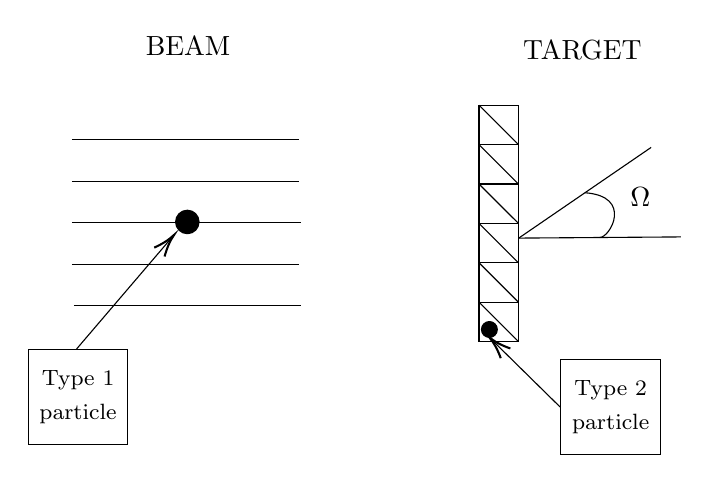
\begin{tikzpicture}[x=0.75pt,y=0.75pt,yscale=-1,xscale=1]
%uncomment if require: \path (0,300); %set diagram left start at 0, and has height of 300
%Straight Lines [id:da7601078847096199] 
\draw    (90,80) -- (199.3,80) ;
%Straight Lines [id:da41431446732450006] 
\draw    (90,100) -- (199.3,100) ;
%Straight Lines [id:da7406610884448859] 
\draw    (90,120) -- (200.3,120) ;
%Straight Lines [id:da5555389414112442] 
\draw    (90,140) -- (199.3,140) ;
%Straight Lines [id:da7113604441316939] 
\draw    (91,160) -- (200.3,160) ;
%Shape: Circle [id:dp6032562484660473] 
\draw  [fill={rgb, 255:red, 0; green, 0; blue, 0 }  ,fill opacity=1 ] (140,119.6) .. controls (140,116.48) and (142.53,113.95) .. (145.65,113.95) .. controls (148.77,113.95) and (151.3,116.48) .. (151.3,119.6) .. controls (151.3,122.72) and (148.77,125.25) .. (145.65,125.25) .. controls (142.53,125.25) and (140,122.72) .. (140,119.6) -- cycle ;
%Straight Lines [id:da4553990376870143] 
\draw    (92.3,180.8) -- (138,127.32) ;
\draw [shift={(139.3,125.8)}, rotate = 490.52] [color={rgb, 255:red, 0; green, 0; blue, 0 }  ][line width=0.75]    (10.93,-3.29) .. controls (6.95,-1.4) and (3.31,-0.3) .. (0,0) .. controls (3.31,0.3) and (6.95,1.4) .. (10.93,3.29)   ;
%Shape: Square [id:dp6385245267322448] 
\draw   (286.2,158.26) -- (305.18,158.26) -- (305.18,177.23) -- (286.2,177.23) -- cycle ;
%Straight Lines [id:da048366194956986464] 
\draw    (286.2,158.26) -- (305.18,177.23) ;
%Shape: Rectangle [id:dp3214112118743824] 
\draw   (286.2,139.28) -- (305.18,139.28) -- (305.18,158.26) -- (286.2,158.26) -- cycle ;
%Straight Lines [id:da08317295232905786] 
\draw    (286.2,139.28) -- (305.18,158.26) ;
%Shape: Square [id:dp9323954113559714] 
\draw   (286.2,120.3) -- (305.18,120.3) -- (305.18,139.28) -- (286.2,139.28) -- cycle ;
%Straight Lines [id:da45254561705281793] 
\draw    (286.2,120.3) -- (305.18,139.28) ;
%Shape: Rectangle [id:dp12155363507098405] 
\draw   (286.2,101.33) -- (305.18,101.33) -- (305.18,120.3) -- (286.2,120.3) -- cycle ;
%Straight Lines [id:da8476758996401002] 
\draw    (286.2,101.33) -- (305.18,120.3) ;
%Shape: Rectangle [id:dp34942394137534416] 
\draw   (286.2,82.35) -- (305.18,82.35) -- (305.18,101.33) -- (286.2,101.33) -- cycle ;
%Straight Lines [id:da38815018499337417] 
\draw    (286.2,82.35) -- (305.18,101.33) ;
%Shape: Ellipse [id:dp6086410383693974] 
\draw  [fill={rgb, 255:red, 0; green, 0; blue, 0 }  ,fill opacity=1 ] (287.37,171.42) .. controls (287.37,169.31) and (289.08,167.6) .. (291.19,167.6) .. controls (293.3,167.6) and (295.01,169.31) .. (295.01,171.42) .. controls (295.01,173.52) and (293.3,175.23) .. (291.19,175.23) .. controls (289.08,175.23) and (287.37,173.52) .. (287.37,171.42) -- cycle ;
%Shape: Rectangle [id:dp006552695566079958] 
\draw   (286.2,63.37) -- (305.18,63.37) -- (305.18,82.35) -- (286.2,82.35) -- cycle ;
%Straight Lines [id:da9936025699051918] 
\draw    (286.2,63.37) -- (305.18,82.35) ;
%Straight Lines [id:da19771769575127984] 
\draw    (325.3,208.8) -- (292.61,176.64) ;
\draw [shift={(291.19,175.23)}, rotate = 404.53999999999996] [color={rgb, 255:red, 0; green, 0; blue, 0 }  ][line width=0.75]    (10.93,-3.29) .. controls (6.95,-1.4) and (3.31,-0.3) .. (0,0) .. controls (3.31,0.3) and (6.95,1.4) .. (10.93,3.29)   ;
%Straight Lines [id:da661445200042976] 
\draw    (305.34,127.38) -- (383.4,126.81) ;
%Straight Lines [id:da0566268996079935] 
\draw    (305.34,127.38) -- (369.12,83.68) ;
%Curve Lines [id:da8769720720143497] 
\draw    (337.23,105.53) .. controls (360.55,107.24) and (349.37,127.1) .. (344.37,127.1) ;
% Text Node
\draw    (69,181) -- (117,181) -- (117,227) -- (69,227) -- cycle  ;
\draw (93,204) node   [align=center] {{{\footnotesize Type 1}}\\{{\footnotesize particle}}};
% Text Node
\draw (146,35) node   [align=center] {{BEAM}};
% Text Node
\draw    (325.62,185.8) -- (373.62,185.8) -- (373.62,231.8) -- (325.62,231.8) -- cycle  ;
\draw (349.62,208.8) node   [align=center] {{{\footnotesize Type 2}}\\{{\footnotesize particle}}};
% Text Node
\draw (363.9,107.39) node    {$\Omega $};
% Text Node
\draw (336,37) node   [align=left] {TARGET};
\end{tikzpicture}
\end{center}

Consider a beam of particles with mass $m_1$, number (assuming a uniform distribution) density $n_1^{(0)}$ (subscript 0 is meant to stress that these are number densities in a specific frame, that with particle 2 at rest) and velocity $v_1$ inpining on a target made of particles with mass $m_2$ and number density $n_2^{(0)}$ at rest.\\
Let $N_s$ be the number of scattering events that place per unit volume and per unit time
\[
\frac{N_t}{T} \phi_1 N_2 \sigma = \bigl( n_1^{(0)} v_1 \bigr) \bigl( n_2^{(0)} V \bigr) \sigma
\]
More formally we have
\[
\de N_s = \sigma v_1 n_1^{(0)} n_2^{(0)} \ \de V \de V
\]
with:
\begin{enumerate}
\item T: unit of time
\item $\phi_1$: flux of the beam $\phi_1 = n_1^{(0)} v_1$
\item $N_2$: particles per unit volume in the detector $N_2 = n_2^{(0)}V$
\item $\sigma$: proportionality constant
\end{enumerate}
Dimensional analysis shows $[\sigma] = [L]^2$ and then $\sigma$, called cross section, can be interpreted as an ``effective area''.

\onlyinmainfile{\end{comment}}
\end{document}